% Одностраничная статья по ВКР.
% Компиляция: xelatex article.tex или lualatex article.tex (TeX Live / MiKTeX; в Overleaf — компилятор XeLaTeX).
% Шрифты: Liberation Serif + Inter; если их нет, подставятся Times New Roman и Liberation Sans / Arial.
% Все иллюстрации нарисованы в TikZ прямо в этом файле — их можно править.
\documentclass[a4paper,10pt]{article}

\usepackage[a4paper,top=8mm,bottom=12mm,left=11mm,right=11mm,footskip=6mm]{geometry}
\usepackage{fontspec}
\usepackage[english]{babel}
\babelprovide[import,main]{russian}
\usepackage{xcolor}
\usepackage{tikz}
\usetikzlibrary{arrows.meta}
\usepackage{multicol}
\usepackage{caption}
\usepackage{booktabs}
\usepackage{tabularx}
\usepackage{tcolorbox}
\tcbuselibrary{skins}
\usepackage{amsmath}
\usepackage{unicode-math}
\usepackage{fancyhdr}
\usepackage[hidelinks]{hyperref}

% --- шрифты: основной текст — Times-подобный, подписи и графика — гротеск
\IfFontExistsTF{Liberation Serif}{\setmainfont{Liberation Serif}}{\setmainfont{Times New Roman}}
\IfFontExistsTF{TeX Gyre Termes Math}{\setmathfont{TeX Gyre Termes Math}}{}
\IfFontExistsTF{Inter}{\setsansfont{Inter}}{\IfFontExistsTF{Liberation Sans}{\setsansfont{Liberation Sans}}{\setsansfont{Arial}}}

% --- палитра
\definecolor{ink}{HTML}{16191D}
\definecolor{ink2}{HTML}{4A525C}
\definecolor{ink3}{HTML}{7A828C}
\definecolor{rule}{HTML}{D5D9DE}
\definecolor{tint}{HTML}{F3F5F8}
\definecolor{pqc}{HTML}{1F57B5}
\definecolor{pqcbg}{HTML}{EEF3FB}
\definecolor{pqclt}{HTML}{DBE6F7}
\definecolor{hyb}{HTML}{D0571B}
\definecolor{hybdk}{HTML}{B0440F}
\definecolor{hybbg}{HTML}{FDF1EA}
\definecolor{base}{HTML}{B9C0C8}
\definecolor{wire}{HTML}{EEF1F4}

% --- плотная вёрстка
\renewcommand\normalsize{\fontsize{8.2}{10.1}\selectfont
  \abovedisplayskip=2pt plus 1pt \belowdisplayskip=2pt plus 1pt
  \abovedisplayshortskip=1pt \belowdisplayshortskip=1pt}
\normalsize
\setlength{\parindent}{3.5mm}
\setlength{\parskip}{0pt}
\setlength{\columnsep}{5.5mm}
\setlength{\columnseprule}{0.3pt}
\setlength{\multicolsep}{1mm}
\renewcommand{\columnseprulecolor}{\color{rule}}
\emergencystretch=1.5em

\captionsetup{font={sf,scriptsize},labelfont={bf,color=ink},textfont={color=ink2},
  labelsep=period,justification=raggedright,singlelinecheck=false,skip=2pt}
\captionsetup[table]{position=top,skip=2pt}

\newcommand{\sect}[2]{\par\vspace{1.4mm}\noindent{\sffamily\bfseries\fontsize{7}{8.5}\selectfont
  \if\relax\detokenize{#1}\relax\else\textcolor{pqc}{#1}\hspace{1.3mm}\fi\MakeUppercase{#2}}\par\nopagebreak\vspace{0.7mm}}
\newcommand{\lbl}[1]{{\sffamily\bfseries\fontsize{6.2}{7}\selectfont\textcolor{pqc}{\MakeUppercase{#1}}}\hspace{1.2mm}}
\newcommand{\stat}[3]{%
  \fcolorbox{rule}{white}{\parbox[t][12mm]{25.4mm}{\raggedright\vspace{0.3mm}%
    {\sffamily\bfseries\fontsize{13}{13}\selectfont\textcolor{#1}{#2}}\\[0.6mm]
    {\sffamily\fontsize{6}{7.2}\selectfont\textcolor{ink2}{#3}\par}}}}

\pagestyle{fancy}
\fancyhf{}
\renewcommand{\headrulewidth}{0pt}
\fancyfoot[L]{\sffamily\fontsize{6.2}{7}\selectfont\textcolor{ink3}{© 2026 М.\,В.~Заславцев · МАИ, кафедра 806}}
\fancyfoot[R]{\sffamily\fontsize{6.2}{7}\selectfont\textcolor{ink3}{Исходный код: \href{https://github.com/MaximusPokeZ/pqc-diploma}{github.com/MaximusPokeZ/pqc-diploma}}}

\begin{document}
\color{ink}

% ================= ШАПКА =================
\noindent{\sffamily\bfseries\fontsize{6.3}{7}\selectfont
  \textcolor{pqc}{ИНФОРМАЦИОННАЯ БЕЗОПАСНОСТЬ · ПОСТКВАНТОВАЯ КРИПТОГРАФИЯ}\hfill
  \textcolor{ink2}{НАУЧНАЯ СТАТЬЯ · УДК 004.056.55}}\\[-1mm]
\textcolor{ink}{\rule{\textwidth}{1.5pt}}

\vspace{2mm}
\noindent{\raggedright\sffamily\bfseries\fontsize{14}{16}\selectfont
Квантово-устойчивое хранение цифровых активов: гибридный KEM X25519 + ML-KEM
и~спектральное предсжатие на~платформе Java~25\par}

\vspace{0.9mm}
\noindent{\itshape\fontsize{7.8}{9.5}\selectfont\textcolor{ink2}{\foreignlanguage{english}{Quantum-resistant storage of digital assets: hybrid X25519 + ML-KEM key encapsulation and spectral pre-compression on Java 25}}\par}

\vspace{1.2mm}
\noindent{\sffamily\fontsize{7.8}{9.5}\selectfont\textbf{М.\,В.~Заславцев}\ \textcolor{ink2}{· науч. рук. — к.\,т.\,н., доцент А.\,М.~Романенков}\par}
\noindent{\sffamily\fontsize{6.8}{8.4}\selectfont\textcolor{ink2}{Московский авиационный институт (НИУ), кафедра 806 «Вычислительная математика и программирование», Москва}\par}

\vspace{2mm}
% ================= АННОТАЦИЯ =================
\begin{tcolorbox}[enhanced jigsaw, colback=tint, colframe=pqc, boxrule=0pt, leftrule=0.8mm, arc=0pt,
  left=3mm, right=2mm, top=1.6mm, bottom=1.6mm, boxsep=0pt, before skip=0pt, after skip=0pt]
  \begin{minipage}[c]{\dimexpr\linewidth-63mm\relax}
    \fontsize{8}{10}\selectfont
    \lbl{Аннотация}Атака «Harvest Now, Decrypt Later» угрожает уже сегодня архивам, которые должны оставаться секретными 10~лет и~более: перехваченный шифротекст будет вскрыт алгоритмом Шора на квантовом компьютере. Предложена подсистема хранения, в~которой ключ данных выводится через HKDF из двух независимых секретов — X25519 и~ML-KEM-768 (FIPS~203), а~целостность обеспечивает композитная подпись Ed25519\,‖\,ML-DSA-65 (FIPS~204). Рост PQC-артефактов компенсирует конвейер «сжатие~→~шифрование» с~авторским спектрально-энтропийным алгоритмом FOURIER. Решение реализовано на штатных API Java~25 как криптоагильный Spring Boot Starter.

    \vspace{1mm}
    {\fontsize{7.3}{9}\selectfont\color{ink2}\lbl{Ключевые слова}постквантовая криптография, ML-KEM, ML-DSA, гибридный KEM, HKDF, HNDL, Compress-then-Encrypt, БПФ, Java~25.}
  \end{minipage}\hfill
  \begin{minipage}[c]{60mm}
    \setlength{\fboxsep}{1.4mm}\setlength{\fboxrule}{0.4pt}
    \stat{pqc}{71\,\%}{сжатие телеметрии алгоритмом FOURIER (ZSTD~— 21\,\%)}\hspace{1.2mm}%
    \stat{hyb}{−29\,\%}{время крипто-цикла при сжатии перед AES-GCM}\\[1.2mm]
    \stat{pqc}{8×}{верификация ML-DSA-65 быстрее, чем Ed25519}\hspace{1.2mm}%
    \stat{hyb}{5\,300}{гибридных операций/с (10~КБ, одно ядро)}
  \end{minipage}
\end{tcolorbox}

\vspace{2mm}
% ================= РИС. 1 — АРХИТЕКТУРА =================
% Координаты в «пикселях» 700×161, ось y направлена вниз.
\noindent\begin{minipage}{\textwidth}
\centering
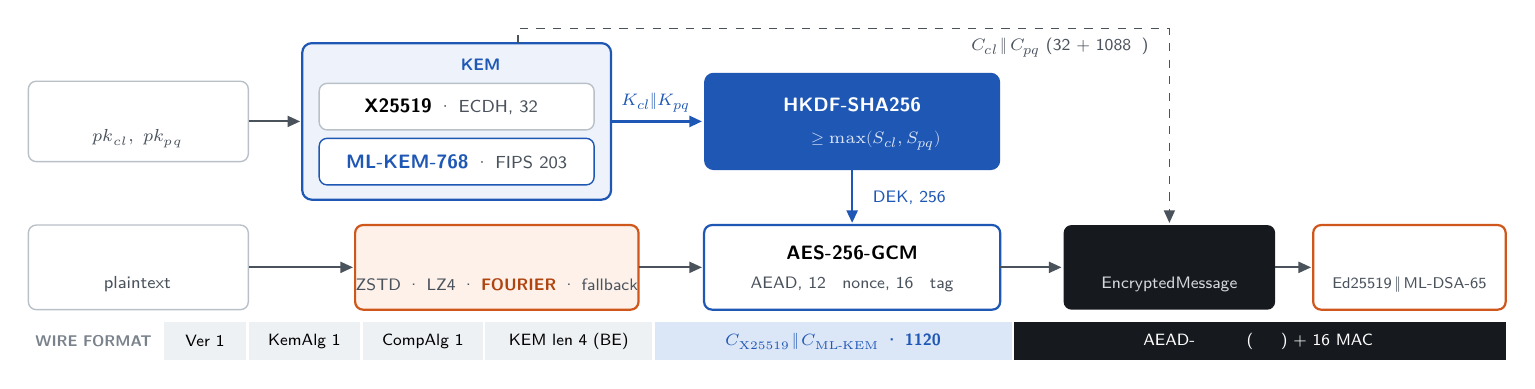
\begin{tikzpicture}[x=0.2686mm, y=-0.2686mm, font=\sffamily\fontsize{7}{8}\selectfont,
  box/.style={draw=base, fill=white, rounded corners=1mm, line width=0.5pt},
  arr/.style={-{Triangle[length=1.6mm,width=1.4mm]}, draw=ink2, line width=0.7pt},
  arrb/.style={-{Triangle[length=1.6mm,width=1.4mm]}, draw=pqc, line width=0.9pt},
  sub/.style={text=ink2, font=\sffamily\fontsize{6.3}{7}\selectfont}]
  % ключ получателя
  \draw[box] (0.5,28) rectangle (104.5,66);
  \node[font=\sffamily\bfseries\fontsize{7}{8}\selectfont] at (52,41) {Ключ получателя};
  \node[sub] at (52,55) {$pk_{cl},\ pk_{pq}$};
  \draw[arr] (105,47) -- (129,47);
  % гибридный KEM
  \draw[draw=pqc, fill=pqcbg, rounded corners=1.2mm, line width=0.8pt] (130,10) rectangle (276,84);
  \node[text=pqc, font=\sffamily\bfseries\fontsize{6}{7}\selectfont] at (203,20) {ГИБРИДНЫЙ KEM};
  \draw[box] (138,29) rectangle (268,51);
  \node at (203,40) {\textbf{X25519}\textcolor{ink2}{\fontsize{6.3}{7}\selectfont\ · ECDH, 32 Б}};
  \draw[box, draw=pqc] (138,55) rectangle (268,77);
  \node at (203,66) {\textcolor{pqc}{\textbf{ML-KEM-768}}\textcolor{ink2}{\fontsize{6.3}{7}\selectfont\ · FIPS 203}};
  % K -> HKDF
  \draw[arrb] (276,47) -- (319,47);
  \node[text=pqc, font=\sffamily\fontsize{6}{7}\selectfont] at (297,38) {$K_{cl}\|K_{pq}$};
  % HKDF
  \fill[pqc, rounded corners=1.2mm] (320,24) rectangle (460,70);
  \node[text=white, font=\sffamily\bfseries\fontsize{7}{8}\selectfont] at (390,39) {HKDF-SHA256};
  \node[text=pqclt, font=\sffamily\fontsize{6}{7}\selectfont] at (390,56) {стойкость $\geq \max(S_{cl}, S_{pq})$};
  % инкапсуляции -> контейнер
  \draw[arr, dashed, line width=0.5pt] (232,10) -- (232,3) -- (540,3) -- (540,95);
  \node[anchor=east, sub, font=\sffamily\fontsize{6}{7}\selectfont] at (534,12) {инкапсуляции $C_{cl}\,\|\,C_{pq}$ (32 + 1088 Б)};
  % DEK
  \draw[arrb] (390,70) -- (390,95);
  \node[anchor=west, text=pqc, font=\sffamily\fontsize{6}{7}\selectfont] at (396,83) {DEK, 256 бит};
  % основной конвейер
  \draw[box] (0.5,96) rectangle (104.5,136);
  \node[font=\sffamily\bfseries\fontsize{7}{8}\selectfont] at (52,110) {Цифровой актив};
  \node[sub] at (52,124) {plaintext};
  \draw[arr] (105,116) -- (154,116);
  \draw[draw=hyb, fill=hybbg, rounded corners=1mm, line width=0.8pt] (155,96) rectangle (289,136);
  \node[text=hybdk, font=\sffamily\bfseries\fontsize{7}{8}\selectfont] at (222,109) {Сжатие};
  \node[sub, font=\sffamily\fontsize{6}{7}\selectfont] at (222,124) {ZSTD · LZ4 · \textcolor{hybdk}{\textbf{FOURIER}} · fallback};
  \draw[arr] (289,116) -- (319,116);
  \draw[box, draw=pqc, line width=0.8pt] (320,96) rectangle (460,136);
  \node[font=\sffamily\bfseries\fontsize{7}{8}\selectfont] at (390,109) {AES-256-GCM};
  \node[sub, font=\sffamily\fontsize{6}{7}\selectfont] at (390,124) {AEAD, 12 Б nonce, 16 Б tag};
  \draw[arr] (460,116) -- (489,116);
  \fill[ink, rounded corners=1mm] (490,96) rectangle (590,136);
  \node[text=white, font=\sffamily\bfseries\fontsize{7}{8}\selectfont] at (540,109) {Контейнер};
  \node[text=rule, font=\sffamily\fontsize{6}{7}\selectfont] at (540,124) {EncryptedMessage};
  \draw[arr] (590,116) -- (607,116);
  \draw[draw=hyb, fill=white, rounded corners=1mm, line width=0.8pt] (608,96) rectangle (699,136);
  \node[font=\sffamily\bfseries\fontsize{7}{8}\selectfont] at (653.5,109) {Подпись};
  \node[sub, font=\sffamily\fontsize{5.6}{7}\selectfont] at (653.5,124) {Ed25519\,‖\,ML-DSA-65};
  % wire format
  \node[anchor=west, text=ink3, font=\sffamily\bfseries\fontsize{5.6}{7}\selectfont] at (0,151) {WIRE FORMAT};
  \begin{scope}[font=\sffamily\fontsize{5.9}{7}\selectfont]
    \foreach \a/\b/\t in {64/104/Ver 1, 104/158/KemAlg 1, 158/216/CompAlg 1, 216/296/KEM len 4 (BE)} {
      \fill[wire] (\a+0.6,142) rectangle (\b-0.6,160);
      \node at ({(\a+\b)/2},151) {\t};
    }
    \fill[pqclt] (296.6,142) rectangle (465.4,160);
    \node[text=pqc] at (381,151) {\textbf{$C_{\mathrm{X25519}}\,\|\,C_{\mathrm{ML\text{-}KEM}}$ · 1120}};
    \fill[ink] (466.6,142) rectangle (699,160);
    \node[text=white] at (582,151) {AEAD-шифротекст (сжатый) + 16 MAC};
  \end{scope}
\end{tikzpicture}
\captionof{figure}{Гибридный конвейер «сжатие~→~шифрование». Ключ данных выводится из двух независимых секретов и~остаётся стойким, пока не взломаны \textit{оба} механизма инкапсуляции; префиксы длины в~заголовке исключают неоднозначность конкатенации. Размеры полей — в~байтах.}
\end{minipage}

\vspace{0.5mm}
\noindent\textcolor{rule}{\rule{\textwidth}{0.4pt}}
\vspace{-1mm}

% ================= ТЕКСТ =================
\begin{multicols}{2}
\sect{1}{Проблема}
Алгоритм Шора~[1] обнуляет стойкость RSA и~ECC. Для данных в~состоянии покоя важна не дата появления квантового компьютера (CRQC), а~модель HNDL: шифротекст, перехваченный сегодня, будет вскрыт завтра. Жизненный цикл аэрокосмических изделий и~их документации — 20–50~лет, что перекрывает прогнозы появления CRQC~[5]. Стандарты FIPS~203/204 утверждены NIST в~2024~г.~[2,~3], но их криптоанализ молод (финалист NIST SIKE был взломан на обычном ПК), поэтому, следуя ANSSI~[6], мы комбинируем классику с~PQC, а~не заменяем её.

\sect{2}{Метод}
\noindent\textbf{Гибридная инкапсуляция.} X25519 и~ML-KEM-768 выполняются независимо, их секреты смешиваются через HKDF~[4]:
\begin{equation}
K = \mathrm{HKDF\text{-}Expand}\bigl(\mathrm{HKDF\text{-}Extract}(salt,\ K_{cl}\,\|\,K_{pq}),\ info\bigr).
\end{equation}
\noindent В~отличие от наивного хеширования конкатенации, (1) даёт $S_{hyb} \geq \max(S_{cl}, S_{pq})$. Подпись — композит $\omega = (\omega_{\mathrm{Ed25519}}, \omega_{\mathrm{ML\text{-}DSA}})$, принимаемый только при валидности обеих частей.

\textbf{Compress-then-Encrypt.} Шифротекст AES-GCM имеет максимальную энтропию и~не сжимается, поэтому сжатие выполняется до шифрования. Если выигрыша нет (архивы, зашифрованные файлы), сжатие отменяется маркером NONE в~заголовке — контейнер не раздувается.

\textbf{Алгоритм FOURIER.} Словарные методы (LZ77) бессильны на плавных градиентах телеметрии. Блок 1024~Б переводится БПФ (radix-2) в~частотную область, сохраняются 8~низших гармоник, обратное БПФ даёт предсказание $\hat{x}$, а~в~поток пишутся невязки $r_i = (x_i - \hat{x}_i) \bmod 256$. Кольцевая 8-битная арифметика даёт строго обратимое восстановление $x_i = (\hat{x}_i + r_i) \bmod 256$ без ветвлений, а~невязки с~низкой энтропией дожимает ZSTD.

\vspace{1mm}
\noindent\begin{minipage}{\linewidth}
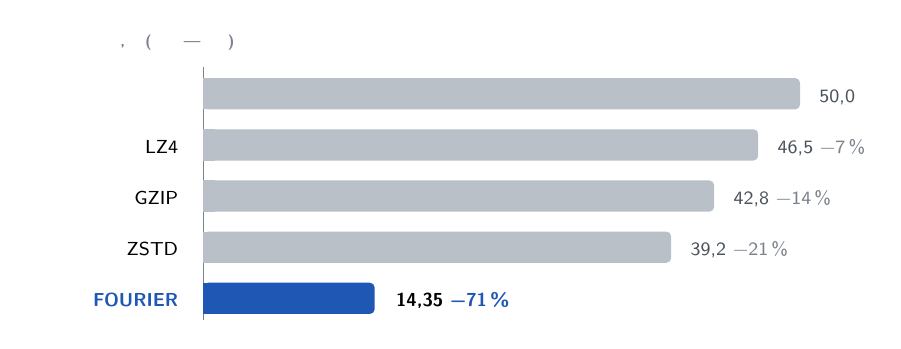
\begin{tikzpicture}[x=\linewidth/336, y=-\linewidth/336, font=\sffamily\fontsize{6.8}{8}\selectfont]
  \node[anchor=base west, text=ink3, font=\sffamily\bfseries\fontsize{5.6}{7}\selectfont] at (0,9) {РАЗМЕР ПОСЛЕ СЖАТИЯ, КБ (МЕНЬШЕ — ЛУЧШЕ)};
  \draw[ink3, line width=0.5pt] (62,16) -- (62,105);
  % 50 КБ = 210 единиц
  \foreach \y/\name/\v/\lab in {20/Исходно/50/{50,0}, 38/LZ4/46.5/{46,5 \textcolor{ink3}{−7\,\%}},
                                56/GZIP/42.8/{42,8 \textcolor{ink3}{−14\,\%}}, 74/ZSTD/39.2/{39,2 \textcolor{ink3}{−21\,\%}}} {
    \node[anchor=base east] at (56,\y+8.5) {\name};
    \fill[base, rounded corners=0.6mm] (62,\y) rectangle ({62+4.2*\v},\y+11);
    \fill[base] (62,\y) rectangle (66,\y+11);
    \node[anchor=base west, text=ink2] at ({62+4.2*\v+4},\y+8.5) {\lab};
  }
  \node[anchor=base east, text=pqc, font=\sffamily\bfseries\fontsize{6.8}{8}\selectfont] at (56,100.5) {FOURIER};
  \fill[pqc, rounded corners=0.6mm] (62,92) rectangle (122.3,103);
  \fill[pqc] (62,92) rectangle (66,103);
  \node[anchor=base west, font=\sffamily\bfseries\fontsize{6.8}{8}\selectfont] at (127,100.5) {14,35 \textcolor{pqc}{−71\,\%}};
\end{tikzpicture}
\captionof{figure}{Сжатие 50~КБ сырой телеметрии с~шумом: нагрузка на AES-GCM ниже в~3,5~раза. На тексте лидирует ZSTD (94,8\,\% против 86,2\,\%), поэтому FOURIER — опция для сигналов.}
\end{minipage}

\sect{3}{Эксперимент}
Замеры выполнены в~демо-приложении на Spring Boot, метрики собирались в~Prometheus и~Grafana (20~итераций после прогрева JIT). Цена квантовой устойчивости — рост артефактов (табл.~1). Контринтуитивно, сжатие \textit{ускоряет} полный крипто-цикл на 29\,\%: компрессия дешевле AEAD-обработки исходного объёма.

\vspace{1mm}
\noindent\begin{minipage}{\linewidth}
\captionof{table}{Цена квантовой устойчивости и~её компенсация}
\sffamily\fontsize{6.7}{8.2}\selectfont
\begin{tabularx}{\linewidth}{@{}X r r@{}}
\toprule
\textcolor{ink2}{Показатель} & \textcolor{ink2}{Классика} & \textcolor{ink2}{Гибрид}\\
\midrule
Накладные расходы KEM, Б & 79 & 1175\\
Размер подписи, Б & 64 & 3309\\
Генерация ключей подписи, мс & 0,4 & 1,8\\
Цикл шифр.+расшифр., мс: без сжатия → LZ4 & — & \textcolor{pqc}{\textbf{0,96 → 0,68}}\\
Пропускная спос-ть, оп/с: без сжатия → LZ4 & 15\,200 & \textcolor{pqc}{\textbf{4100 → 5300}}\\
\bottomrule
\end{tabularx}
\end{minipage}

\vspace{1.5mm}
\noindent\begin{minipage}{\linewidth}
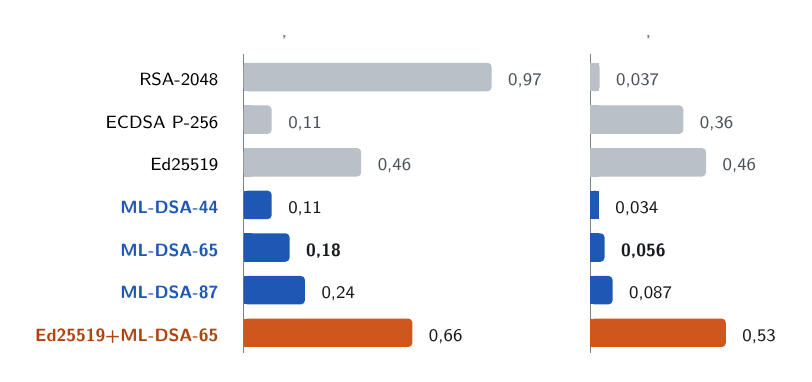
\begin{tikzpicture}[x=\linewidth/336, y=-\linewidth/336, font=\sffamily\fontsize{6.4}{8}\selectfont]
  \node[anchor=base west, text=ink3, font=\sffamily\bfseries\fontsize{5.6}{7}\selectfont] at (104,27) {ПОДПИСЬ, МС};
  \node[anchor=base west, text=ink3, font=\sffamily\bfseries\fontsize{5.6}{7}\selectfont] at (226,27) {ВЕРИФИКАЦИЯ, МС};
  \draw[ink3, line width=0.5pt] (104,33) -- (104,138);
  \draw[ink3, line width=0.5pt] (226,33) -- (226,138);
  % 1 мс = 90 единиц; строки через 15 единиц
  \foreach \i/\name/\col/\s/\sl/\v/\vl in {
      0/RSA-2048/base/0.97/{0,97}/0.0367/{0,037},
      1/ECDSA P-256/base/0.11/{0,11}/0.364/{0,36},
      2/Ed25519/base/0.46/{0,46}/0.453/{0,46},
      3/\textcolor{pqc}{\textbf{ML-DSA-44}}/pqc/0.11/{\textcolor{ink}{0,11}}/0.0338/{\textcolor{ink}{0,034}},
      4/\textcolor{pqc}{\textbf{ML-DSA-65}}/pqc/0.18/{\textcolor{ink}{\textbf{0,18}}}/0.056/{\textcolor{ink}{\textbf{0,056}}},
      5/\textcolor{pqc}{\textbf{ML-DSA-87}}/pqc/0.24/{\textcolor{ink}{0,24}}/0.0874/{\textcolor{ink}{0,087}},
      6/\textcolor{hybdk}{\textbf{Ed25519+ML-DSA-65}}/hyb/0.66/{\textcolor{ink}{0,66}}/0.53/{\textcolor{ink}{0,53}}} {
    \pgfmathsetmacro{\y}{36+15*\i}
    \node[anchor=base east] at (98,\y+8) {\name};
    \fill[\col, rounded corners=0.5mm] (104,\y) rectangle ({104+90*\s},\y+10);
    \fill[\col] (104,\y) rectangle ({104+min(3,90*\s)},\y+10);
    \node[anchor=base west, text=ink2] at ({104+90*\s+3},\y+8) {\sl};
    \fill[\col, rounded corners=0.5mm] (226,\y) rectangle ({226+90*\v},\y+10);
    \fill[\col] (226,\y) rectangle ({226+min(3,90*\v)},\y+10);
    \node[anchor=base west, text=ink2] at ({226+90*\v+3},\y+8) {\vl};
  }
\end{tikzpicture}
\captionof{figure}{Задержки подписи и~верификации: \textcolor{ink3}{классика}, \textcolor{pqc}{PQC}, \textcolor{hybdk}{гибрид}. ML-DSA-65 подписывает в~5~раз быстрее RSA-2048 и~проверяет в~8~раз быстрее Ed25519.}
\end{minipage}

\sect{4}{Заключение}
Создан готовый к~внедрению \textit{pqc-hybrid-spring-boot-starter} на штатных API Java~25 без нативных библиотек~[7]. Режим (HYBRID / PQC\_ONLY / CLASSICAL\_ONLY), уровни ML-KEM и~ML-DSA и~алгоритм сжатия задаются конфигурацией без перекомпиляции — это путь к~будущим отечественным стандартам. Рост артефактов компенсируется предсжатием, а~подпись на решётках быстрее классической.

\sect{}{Литература}
{\fontsize{6.5}{7.9}\selectfont\color{ink2}
\noindent\hangindent=3.5mm\makebox[3.5mm][l]{1.}Shor P.\,W. Algorithms for quantum computation // Proc. 35th FOCS. 1994. P.~124–134.\par
\noindent\hangindent=3.5mm\makebox[3.5mm][l]{2.}NIST FIPS 203: ML-KEM Standard. 2024.\par
\noindent\hangindent=3.5mm\makebox[3.5mm][l]{3.}NIST FIPS 204: ML-DSA Standard. 2024.\par
\noindent\hangindent=3.5mm\makebox[3.5mm][l]{4.}Krawczyk H., Eronen P. RFC 5869: HKDF. IETF, 2010.\par
\noindent\hangindent=3.5mm\makebox[3.5mm][l]{5.}Mosca M., Piani M. Quantum Threat Timeline Report. Global Risk Institute, 2024.\par
\noindent\hangindent=3.5mm\makebox[3.5mm][l]{6.}ANSSI views on the PQC transition. ANSSI, 2023.\par
\noindent\hangindent=3.5mm\makebox[3.5mm][l]{7.}OpenJDK. JEP 496: ML-KEM; JEP 497: ML-DSA. 2025.\par
}
\end{multicols}

\end{document}
